\chapter{Messprinzip mit Skizze und Versuchsablauf}
\begin{center}
    		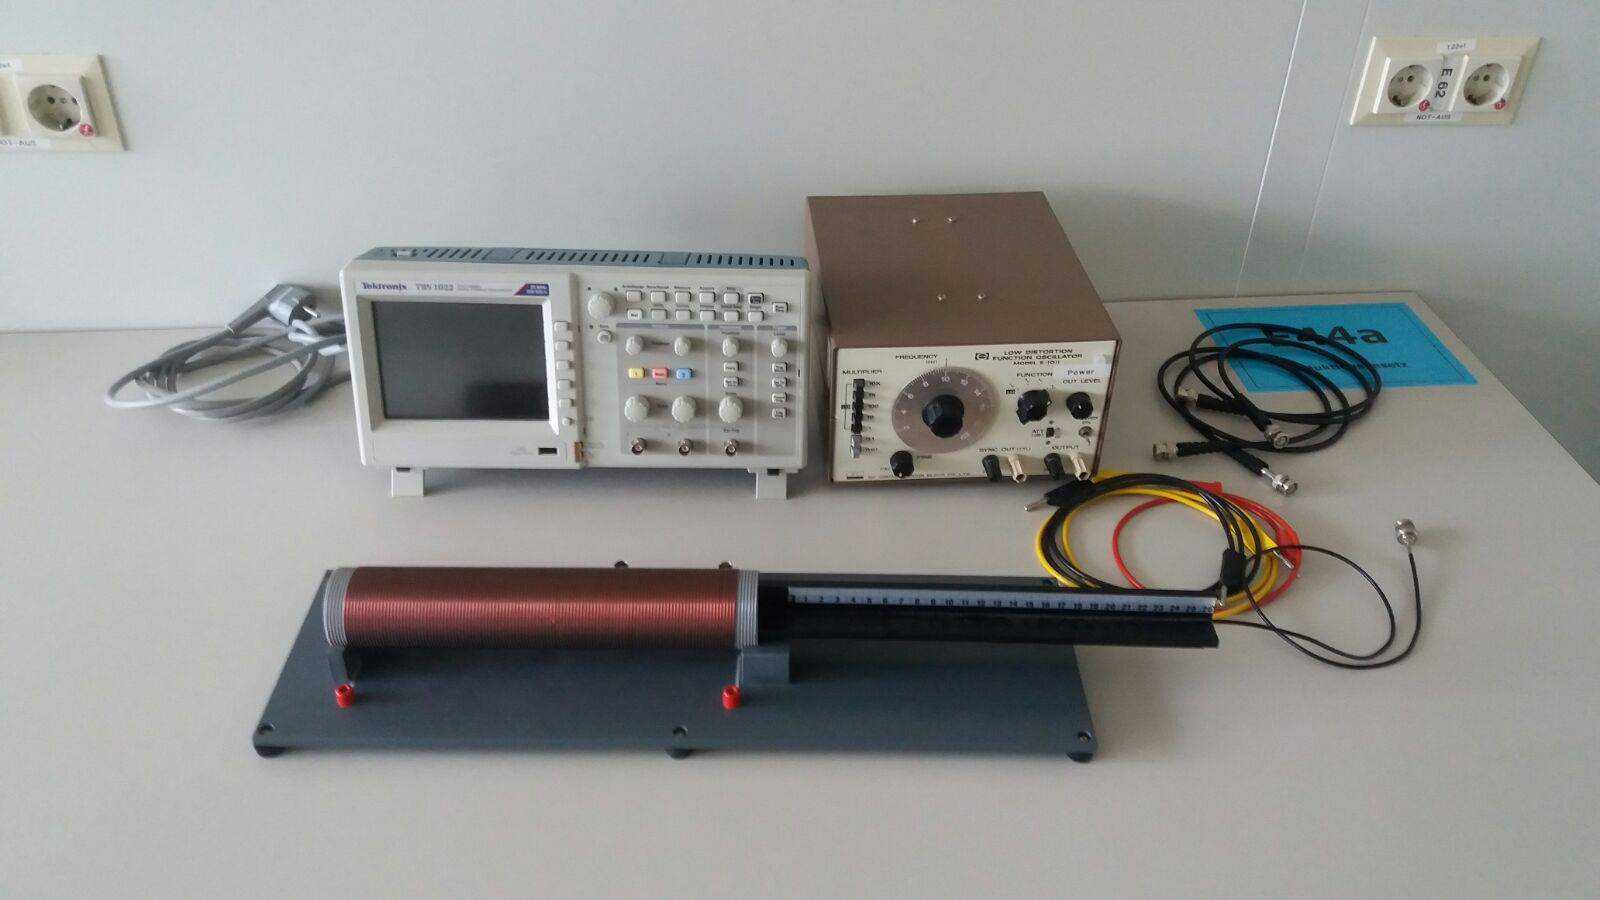
\includegraphics[scale=0.25]{Daten/Aufbau.jpeg}
    	\end{center}
    	\captionof{figure}[]{Versuchsaufbau}
        
        \section{1.Versuchsteil}
        Im ersten Versuchsteil wird das Verhältnis von Eingangsspannung $(U_e)$ zur Ausgangsspannung $(U_a)$ untersucht. Hierfür wird die Frequenz des Stroms nach und nach hochgedreht und dabei die jeweiligen Spannungen bei den jeweiligen Frequenzen notiert.\\
        \\
        \section{2.Versuchsteil}
        Im zweiten Versuchtsteil geht es um die Bestimmung der induzierten Spannung. Hierfür wird eine kleine Spule in eine größere Spule geführt. An der kleinen Spule wird die Spannung gemessen. Die induzierte Spannung wird immer notiert, sobald die kleine Spule 1 cm weiter in die große Spule geschoben wird. Die große Spule hat  eine Länge von 12,5 cm. Es wird auch weiter außerhalb der Spule gemessen.\\
        \\
        \section{3.Versuchsteil}
        In diesem Versuchsteil geht es um die Bestimmung der in der kleinen Spule induzierten Spannung bei unterschiedlichen Frequenzen. Hierfür wird die kleine Spule in die Mitte der großen Spule geschoben und dort gelassen. Die Frequenz wird nach und nach nach oben gedreht und die jeweils induzierten Spannungen notiert.\\
        \\
        \section{4.Versuchsteil}
        Hierfür werden verschiedene Eingangsspannungen an die äußere Spule angelegt. Über einen Oszilloskop wird die Ausgangsspannung beobachtet.\\
        \\
        \section{5. Versuchsteil}
        Im letzten Versuchsteil wird eine Rechtseckspannung angelegt. Die Frequenz wird auf \   1 kHz eingestellt. Die Spule wird kurzgeschlossen und die Ausgangsspannung beobachtet.
        
\pagebreak